% Options for packages loaded elsewhere
\PassOptionsToPackage{unicode}{hyperref}
\PassOptionsToPackage{hyphens}{url}
\PassOptionsToPackage{dvipsnames,svgnames,x11names}{xcolor}
%
\documentclass[
  letterpaper,
  DIV=11,
  numbers=noendperiod]{scrartcl}

\usepackage{amsmath,amssymb}
\usepackage{lmodern}
\usepackage{iftex}
\ifPDFTeX
  \usepackage[T1]{fontenc}
  \usepackage[utf8]{inputenc}
  \usepackage{textcomp} % provide euro and other symbols
\else % if luatex or xetex
  \usepackage{unicode-math}
  \defaultfontfeatures{Scale=MatchLowercase}
  \defaultfontfeatures[\rmfamily]{Ligatures=TeX,Scale=1}
\fi
% Use upquote if available, for straight quotes in verbatim environments
\IfFileExists{upquote.sty}{\usepackage{upquote}}{}
\IfFileExists{microtype.sty}{% use microtype if available
  \usepackage[]{microtype}
  \UseMicrotypeSet[protrusion]{basicmath} % disable protrusion for tt fonts
}{}
\makeatletter
\@ifundefined{KOMAClassName}{% if non-KOMA class
  \IfFileExists{parskip.sty}{%
    \usepackage{parskip}
  }{% else
    \setlength{\parindent}{0pt}
    \setlength{\parskip}{6pt plus 2pt minus 1pt}}
}{% if KOMA class
  \KOMAoptions{parskip=half}}
\makeatother
\usepackage{xcolor}
\setlength{\emergencystretch}{3em} % prevent overfull lines
\setcounter{secnumdepth}{5}
% Make \paragraph and \subparagraph free-standing
\ifx\paragraph\undefined\else
  \let\oldparagraph\paragraph
  \renewcommand{\paragraph}[1]{\oldparagraph{#1}\mbox{}}
\fi
\ifx\subparagraph\undefined\else
  \let\oldsubparagraph\subparagraph
  \renewcommand{\subparagraph}[1]{\oldsubparagraph{#1}\mbox{}}
\fi


\providecommand{\tightlist}{%
  \setlength{\itemsep}{0pt}\setlength{\parskip}{0pt}}\usepackage{longtable,booktabs,array}
\usepackage{calc} % for calculating minipage widths
% Correct order of tables after \paragraph or \subparagraph
\usepackage{etoolbox}
\makeatletter
\patchcmd\longtable{\par}{\if@noskipsec\mbox{}\fi\par}{}{}
\makeatother
% Allow footnotes in longtable head/foot
\IfFileExists{footnotehyper.sty}{\usepackage{footnotehyper}}{\usepackage{footnote}}
\makesavenoteenv{longtable}
\usepackage{graphicx}
\makeatletter
\def\maxwidth{\ifdim\Gin@nat@width>\linewidth\linewidth\else\Gin@nat@width\fi}
\def\maxheight{\ifdim\Gin@nat@height>\textheight\textheight\else\Gin@nat@height\fi}
\makeatother
% Scale images if necessary, so that they will not overflow the page
% margins by default, and it is still possible to overwrite the defaults
% using explicit options in \includegraphics[width, height, ...]{}
\setkeys{Gin}{width=\maxwidth,height=\maxheight,keepaspectratio}
% Set default figure placement to htbp
\makeatletter
\def\fps@figure{htbp}
\makeatother
\newlength{\cslhangindent}
\setlength{\cslhangindent}{1.5em}
\newlength{\csllabelwidth}
\setlength{\csllabelwidth}{3em}
\newlength{\cslentryspacingunit} % times entry-spacing
\setlength{\cslentryspacingunit}{\parskip}
\newenvironment{CSLReferences}[2] % #1 hanging-ident, #2 entry spacing
 {% don't indent paragraphs
  \setlength{\parindent}{0pt}
  % turn on hanging indent if param 1 is 1
  \ifodd #1
  \let\oldpar\par
  \def\par{\hangindent=\cslhangindent\oldpar}
  \fi
  % set entry spacing
  \setlength{\parskip}{#2\cslentryspacingunit}
 }%
 {}
\usepackage{calc}
\newcommand{\CSLBlock}[1]{#1\hfill\break}
\newcommand{\CSLLeftMargin}[1]{\parbox[t]{\csllabelwidth}{#1}}
\newcommand{\CSLRightInline}[1]{\parbox[t]{\linewidth - \csllabelwidth}{#1}\break}
\newcommand{\CSLIndent}[1]{\hspace{\cslhangindent}#1}

\KOMAoption{captions}{tableheading}
\makeatletter
\makeatother
\makeatletter
\makeatother
\makeatletter
\@ifpackageloaded{caption}{}{\usepackage{caption}}
\AtBeginDocument{%
\ifdefined\contentsname
  \renewcommand*\contentsname{Indice de contenidos}
\else
  \newcommand\contentsname{Indice de contenidos}
\fi
\ifdefined\listfigurename
  \renewcommand*\listfigurename{Listado de Figuras}
\else
  \newcommand\listfigurename{Listado de Figuras}
\fi
\ifdefined\listtablename
  \renewcommand*\listtablename{Listado de Tablas}
\else
  \newcommand\listtablename{Listado de Tablas}
\fi
\ifdefined\figurename
  \renewcommand*\figurename{Figura}
\else
  \newcommand\figurename{Figura}
\fi
\ifdefined\tablename
  \renewcommand*\tablename{Tabla}
\else
  \newcommand\tablename{Tabla}
\fi
}
\@ifpackageloaded{float}{}{\usepackage{float}}
\floatstyle{ruled}
\@ifundefined{c@chapter}{\newfloat{codelisting}{h}{lop}}{\newfloat{codelisting}{h}{lop}[chapter]}
\floatname{codelisting}{Listado}
\newcommand*\listoflistings{\listof{codelisting}{Listado de Listatdos}}
\makeatother
\makeatletter
\@ifpackageloaded{caption}{}{\usepackage{caption}}
\@ifpackageloaded{subcaption}{}{\usepackage{subcaption}}
\makeatother
\makeatletter
\@ifpackageloaded{tcolorbox}{}{\usepackage[many]{tcolorbox}}
\makeatother
\makeatletter
\@ifundefined{shadecolor}{\definecolor{shadecolor}{rgb}{.97, .97, .97}}
\makeatother
\makeatletter
\makeatother
\ifLuaTeX
\usepackage[bidi=basic]{babel}
\else
\usepackage[bidi=default]{babel}
\fi
\babelprovide[main,import]{spanish}
% get rid of language-specific shorthands (see #6817):
\let\LanguageShortHands\languageshorthands
\def\languageshorthands#1{}
\ifLuaTeX
  \usepackage{selnolig}  % disable illegal ligatures
\fi
\IfFileExists{bookmark.sty}{\usepackage{bookmark}}{\usepackage{hyperref}}
\IfFileExists{xurl.sty}{\usepackage{xurl}}{} % add URL line breaks if available
\urlstyle{same} % disable monospaced font for URLs
\hypersetup{
  pdftitle={Plantilla en Quarto},
  pdfauthor={Emmanuel Alcalá},
  pdflang={es},
  colorlinks=true,
  linkcolor={blue},
  filecolor={Maroon},
  citecolor={Blue},
  urlcolor={Blue},
  pdfcreator={LaTeX via pandoc}}

\title{Plantilla en Quarto}
\author{Emmanuel Alcalá}
\date{14/07/2022}

\begin{document}
\maketitle
\ifdefined\Shaded\renewenvironment{Shaded}{\begin{tcolorbox}[breakable, boxrule=0pt, frame hidden, sharp corners, enhanced, interior hidden, borderline west={3pt}{0pt}{shadecolor}]}{\end{tcolorbox}}\fi

Requerimientos para usar Quarto

\begin{enumerate}
\def\labelenumi{\arabic{enumi}.}
\tightlist
\item
  \href{https://quarto.org/docs/get-started/}{Instalar quarto}
\item
  Instalar un editor de texto. Recomiendo
  \href{https://quarto.org/docs/get-started/hello/vscode.html}{VScode}.
  Si es en VScode, instalar la
  \href{https://marketplace.visualstudio.com/items?itemName=quarto.quarto}{extensión}.
\end{enumerate}

\begin{itemize}
\tightlist
\item
  Para usar con RStudio, ver
  \href{https://quarto.org/docs/get-started/hello/rstudio.html}{aquí}.
\end{itemize}

\begin{enumerate}
\def\labelenumi{\arabic{enumi}.}
\setcounter{enumi}{2}
\tightlist
\item
  Si se va a trabajar con Python debe configurarse apropiadamente. En
  VScode seleccionar el intérprete de Python que se quiere usar (e.g.,
  de conda).
\item
  Para renderizar en pdf debe instalarse \texttt{tinytex}. Abrir
  terminal y escribir
\end{enumerate}

\texttt{quarto\ tools\ install\ tinytex}

\hypertarget{tuxedtulo}{%
\section{Título}\label{tuxedtulo}}

El título de tu projecto. Debe ser conciso y reflejar el argumento
principal. En ocasiones es bueno plantearlo como pregunta, otras veces
como una afirmación.

\hypertarget{introducciuxf3n}{%
\section{Introducción}\label{introducciuxf3n}}

Para estructurar un proyecto por primera vez es recomendable seguir
alguna estructura particular, estandarizada.

La aplicación
\href{https://drivendata.github.io/cookiecutter-data-science/}{Coockiecutter}
provee una estructura estándar que parece adecuada para esto.

Para algunos ejemplos de reportes técnicos de proyectos, revisa los
proyectos finales del curso CS229: Machine Learning de Standford.

\begin{itemize}
\tightlist
\item
  \href{http://cs229.stanford.edu/proj2021spr/}{2021}.
\item
  \href{http://cs229.stanford.edu/proj2019aut/}{2019}.
\item
  \href{http://cs229.stanford.edu/projects2014.html}{2014}.
\end{itemize}

\hypertarget{definiciuxf3n-del-problema-o-pregunta}{%
\subsection{Definición del problema o
pregunta}\label{definiciuxf3n-del-problema-o-pregunta}}

De acuerdo con la primera sesión.

\hypertarget{datos}{%
\section{Datos}\label{datos}}

Aquí describes los datos que usaste, sus fuentes, variables, etc. Deberá
contener la siguiente información:

\begin{enumerate}
\def\labelenumi{\arabic{enumi}.}
\tightlist
\item
  Justificación concisa de por qué el conjunto de datos elegido es
  relevanta para el problema elegido.
\item
  Describir las fuentes de los datos.
\item
  Describir qué procesamiento se hizo para dejarlos en estado usable.
\item
  Describir las variables que contienen los datos (e.g., codebook, en
  caso de que se usen abreviaturas para las variables).
\end{enumerate}

\hypertarget{muxe9todos-y-anuxe1lisis}{%
\section{Métodos y Análisis}\label{muxe9todos-y-anuxe1lisis}}

La figura Figura~\ref{fig-ml} muestra el proceso que estaremos siguiendo
en esta fase.

\emph{IDI-III tratará principamente de estudiar el problema, limpiar y
transformar los datos y seleccionar las variables}, pero también
comenzaremos a escribir y familiarizarnos con las herramientas de
publicación (en este caso, Quarto).

\begin{figure}[h]

{\centering 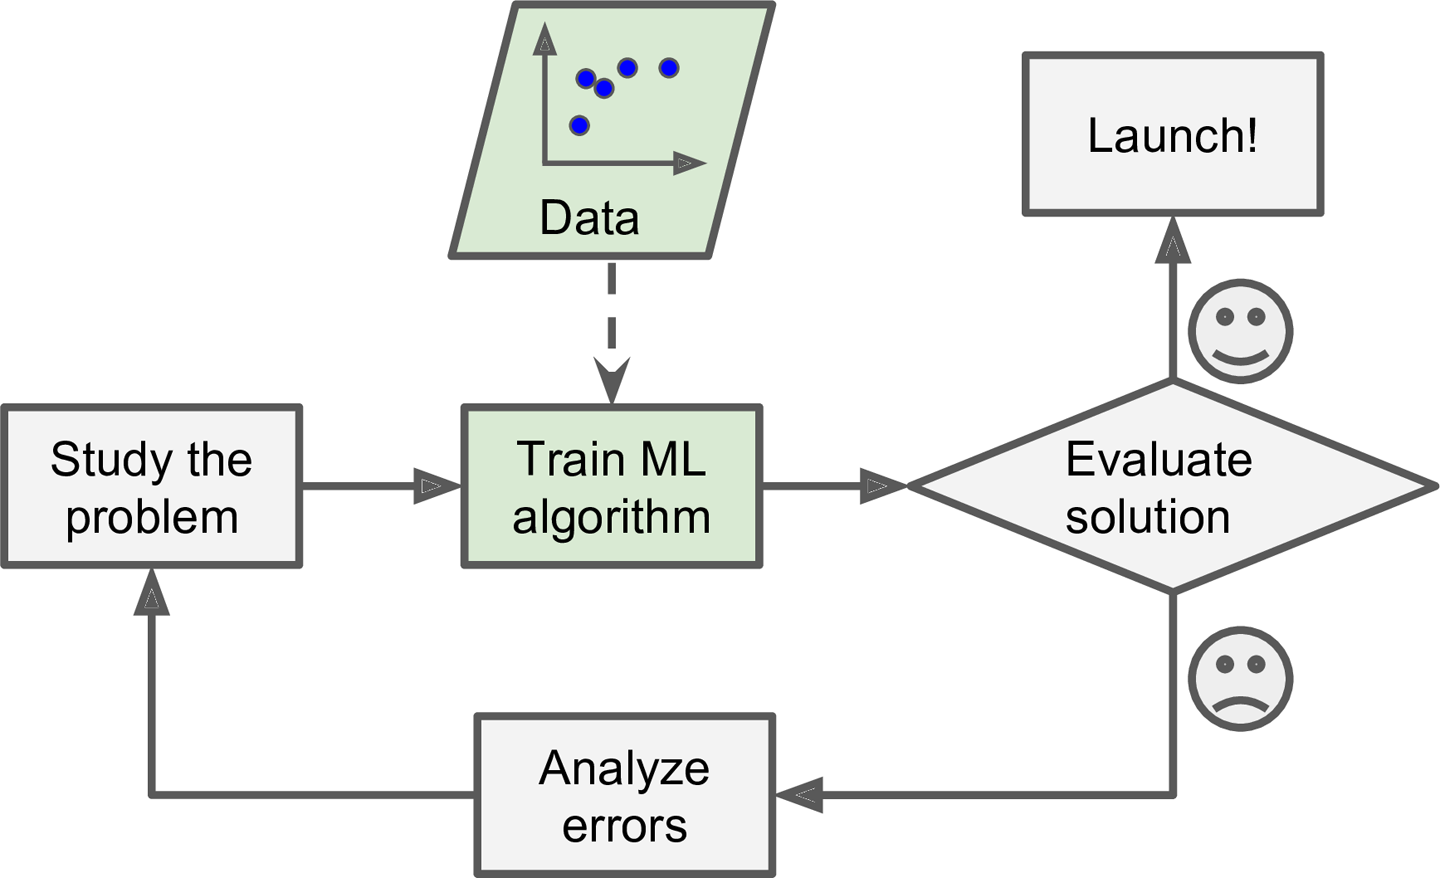
\includegraphics{figs/ml_approach.png}

}

\caption{\label{fig-ml}Proceso típico de proyecto de DS. Tomado de Géron
(2019).}

\end{figure}

\begin{enumerate}
\def\labelenumi{\arabic{enumi}.}
\tightlist
\item
  Análisis exploratorio. Añadir tablas, gráficos exploratorios, etc.
  Esto no es propiamente un resultado, sino un análisis que se realiza
  para justificar otras decisiones.
\item
  Si se realizan transformaciones en una variable (e.g., se
  log-transformó, se exponenció, se escaló, se normalizó, etc) o
  cualquier ingeniería de características, extracción, etc., a partir de
  los datos exploratorios. Justificar la decisión.
\item
  Descripción de los métodos, como algoritmos, benchmarks, métricas de
  comparación (e.g., \(RMSE\)) etc. \emph{No se colocan esos resultados
  aquí}, solo se menciona qu+e se utilizó.
\end{enumerate}

Quarto soporta renderización de ecuaciones usando la sintaxis de \LaTeX.
Ver este
\href{https://quarto.org/docs/authoring/markdown-basics.html\#equations}{artículo}
y \href{https://qmd4sci.njtierney.com/math.html}{este} para ver cómo
escribir matemáticas.

\hypertarget{resultados}{%
\section{Resultados}\label{resultados}}

En esta sección se colocan los resultados principales, como tablas de
comparación, gráficos, etc. Por ejemplo, si se probó un algoritmo con
respecto a otros tres, se coloca la ejecución en diversas métricas.

Las figuras y tablas deben ir acompañadas de una etiqueta y una breve
descripción. Se pueden referenciar usando \texttt{@\{label\}} en donde
\texttt{label} en este caso específico es \texttt{fig-polar}. La
referencia renderizada se verá así Figura~\ref{fig-polar}.

\begin{figure}[h]

{\centering 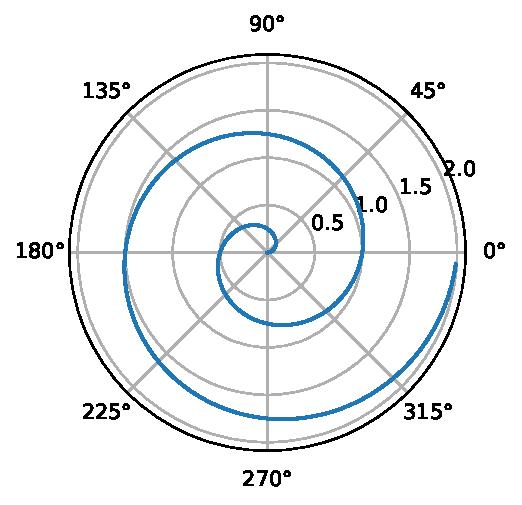
\includegraphics{template_reporte_files/figure-pdf/fig-polar-output-1.pdf}

}

\caption{\label{fig-polar}Esta es la leyenda de una figura.}

\end{figure}

Las tablas pueden hacerse con Markdown

\hypertarget{tbl-letters}{}
\begin{longtable}[]{@{}lll@{}}
\caption{\label{tbl-letters}Leyenda de tabla}\tabularnewline
\toprule()
Col1 & Col2 & Col3 \\
\midrule()
\endfirsthead
\toprule()
Col1 & Col2 & Col3 \\
\midrule()
\endhead
A & B & C \\
E & F & G \\
A & G & G \\
\bottomrule()
\end{longtable}

Ver la tabla Tabla~\ref{tbl-letters}.

\hypertarget{referencias}{%
\section{Referencias}\label{referencias}}

Para citar, usar \texttt{(@alcala2021statistical)} que se renderiza como
(López-Cárdenas et~al. (2021)). La entrada
\texttt{@alcala2021statistical} debe estar tal cual en el archivo
\texttt{referencias.bib}. Las referencias en formato de bibtex se pueden
obtener desde Google Scholar.

Para imprimir las referencias hay que colocar

\begin{verbatim}
::: {#refs}
:::
\end{verbatim}

\hypertarget{refs}{}
\begin{CSLReferences}{1}{0}
\leavevmode\vadjust pre{\hypertarget{ref-geron2019hands}{}}%
Géron, A. (2019). \emph{Hands-on machine learning with Scikit-Learn,
Keras, and TensorFlow: Concepts, tools, and techniques to build
intelligent systems}. O'Reilly Media.

\leavevmode\vadjust pre{\hypertarget{ref-alcala2021statistical}{}}%
López-Cárdenas, P. G., Alcalá, E., Sánchez-Torres, J. D., \& Araujo, E.
(2021). A Resampling Approach for the Data-Based Optimization of
Nanosensors. \emph{2021 18th International Conference on Electrical
Engineering, Computing Science and Automatic Control (CCE)}, 1-4.
\url{https://doi.org/10.1109/CCE53527.2021.9633114}

\end{CSLReferences}



\end{document}
